ReversiXT ist eine Erweiterung des Brettspiels Reversi, welches in den 1880er Jahren vom Engl\"ander Lewis Waterman\footnote{epubli: Reversi/Othello, \textit{https://archive.org/details/reversi.qb64} (abgerufen am 14.05.2021)} entwickelt wurde.
Es handelt sich um ein 2-Personen-Spiel mit einem 8x8 gro"sen Spielfeld.
Es werden je zwei Spielsteine in unterschiedlichen Farben diagonal zueinander mittig auf dem Spielfeld platziert (siehe Abbildung~\ref{fig:basicgame}).
Der rote Spieler beginnt und darf nun auf leere Felder setzen, die ausgehend von diesem Feld in beliebiger Richtung (senkrecht, waagerecht oder diagonal) einen oder mehrere gegnerische Steine zwischen eigenen Steinen einschlie"sen.
Beim Durchf\"uhren eines Spielzuges werden die gegnerischen Spielsteine in die eigene Farbe umgef\"arbt.
Die m\"oglichen Startz\"uge sind in der Grafik semi-transparent eingezeichnet.
Sobald beide Spieler keine Spielz\"uge mehr haben, ist das Spiel beendet.
Gewonnen hat derjenige, der die meisten Steine besitzt.

\vspace{1em}
\begin{minipage}{\linewidth}
	\centering
	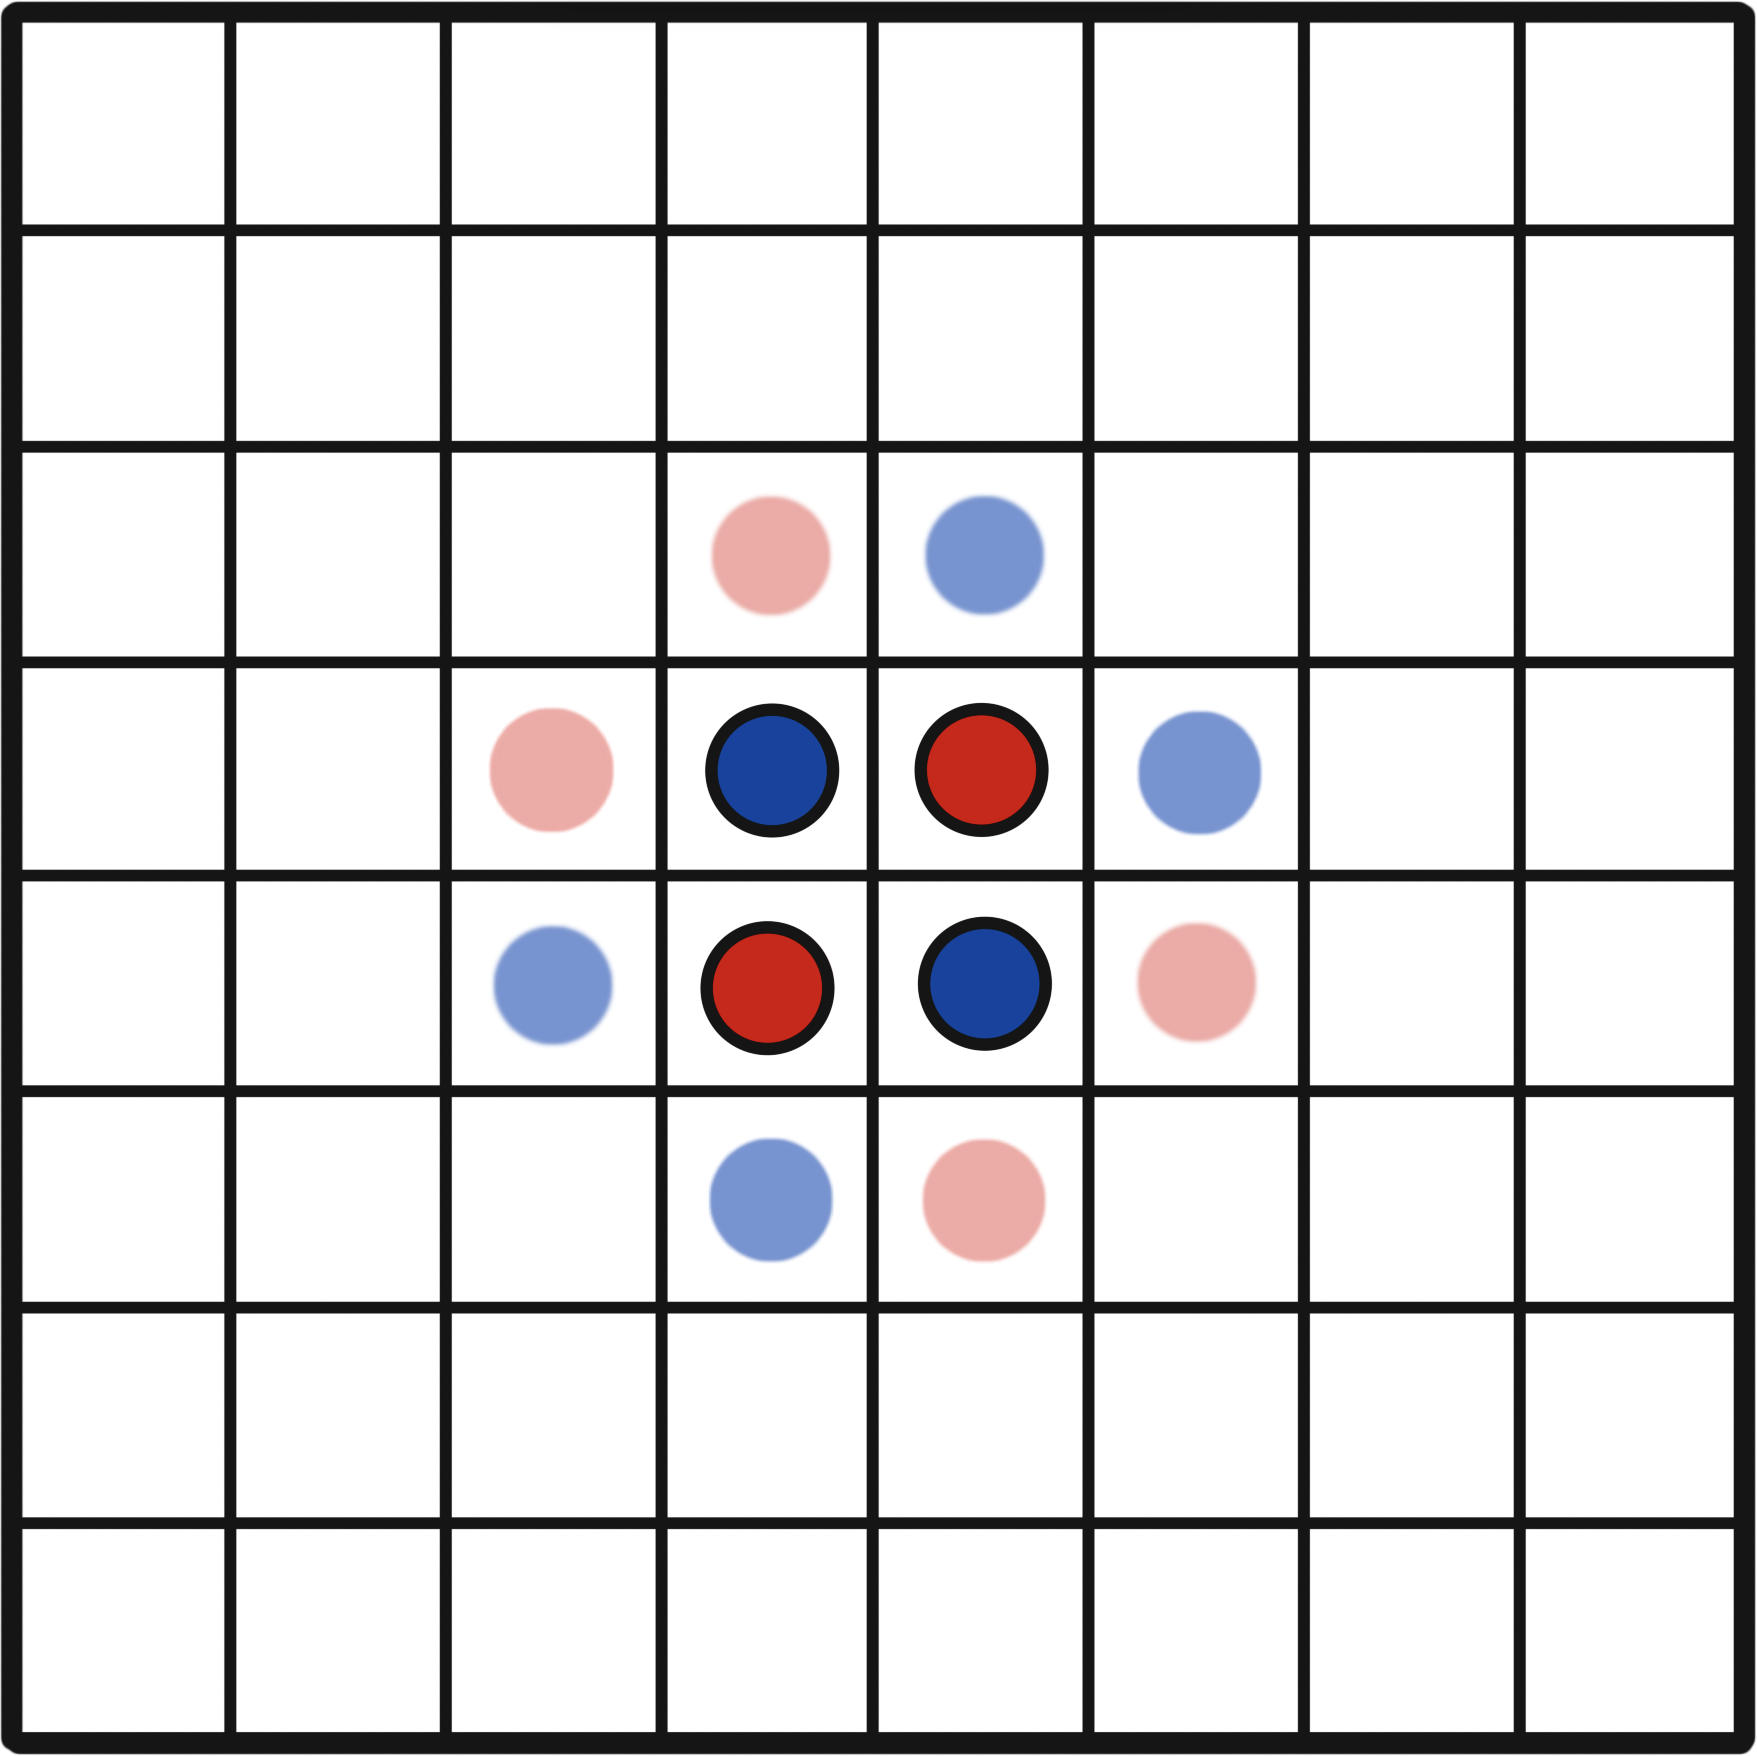
\includegraphics[width=0.5\linewidth]{pics/basicgame-start}
	\captionof{figure}[Grundspiel Start]{Grundspiel Reversi mit möglichen Startzügen (semi-transparent markiert)}
	\label{fig:basicgame}
\end{minipage}

\subsection{Besonderheiten von ReversiXT}\label{subsec:besonderheiten-von-reversixt}
Das Spiel ReversiXT, welches als \emph{Reversi Extreme} bezeichnet wird, basiert auf den gleichen Regeln wie das Grundspiel Reversi.
Es beinhaltet jedoch einige Zusatzregelungen, welche hier kurz erkl\"art werden.
Bei ReversiXT treten bis zu acht Spieler auf einem maximal 50x50 gro"sen Spielfeld gegeneinander an.
Das Spiel besteht dabei aus zwei unterschiedlichen Spielphasen.
In Phase 1 m\"ussen Spieler solange ziehen, bis kein Zug mehr m\"oglich ist.
Im Anschluss beginnt die Phase 2, die sogenannte \emph{Bombenphase}.
Zudem gibt es mehrere Spezialfelder (siehe Abbildung~\ref{fig:reversixt-map}), die vorab fest definiert sind und jeweils nur einmal ausgel\"ost werden k\"onnen.
Mit einem \emph{Inversionsfeld} werden die Farben aller Spieler um eins weiter verschoben.
Mit einem \emph{Choicefeld} wird die Farbe von sich selbst mit einem ausgew\"ahlten Spieler getauscht, dabei ist es auch erlaubt sich selbst zu w\"ahlen.
Ein \emph{Expansionsfeld} wird als Gegner gewertet und kann nach den gleichen Regeln wie andere Spieler eingenommen werden, oder mithilfe eines \emph{\"Uberschreibsteins} - ohne Notwendigkeit der Umf\"arbung anderer Spieler - \"uberschrieben werden.
\"Uberschreibsteine k\"onnen auch genutzt werden, um einen Gegenspieler unter Beachtung der normalen Regeln zu \"uberschreiben und dabei das Spielfeld auf gewohnte Weise einzuf\"arben.
Die Anzahl von \"Uberschreibsteinen sowie Bomben ist zu Beginn des Spieles festgelegt.
Durch ein \emph{Bonusfeld} darf der Spieler zwischen einem \"Uberschreibstein und einer Bombe w\"ahlen, welche dem jeweiligen Spieler gutgeschrieben wird.
Sobald kein Spieler mehr einen legitimen Spielzug besitzt, beginnt die zweite Phase.
Hierbei m\"ussen abwechselnd, sofern vorhanden, alle Bomben gesetzt werden.
Hierzu wird ein Feld ausgew\"ahlt und ein Bereich mit festgelegtem Radius weggesprengt.
Dabei werden alle betroffenen Felder zu L\"ochern umgewandelt.
L\"ocher sind nicht besetzbare Felder, sozusagen nicht bespielbare Felder.

\vspace{1em}
\begin{minipage}{\linewidth}
	\centering
	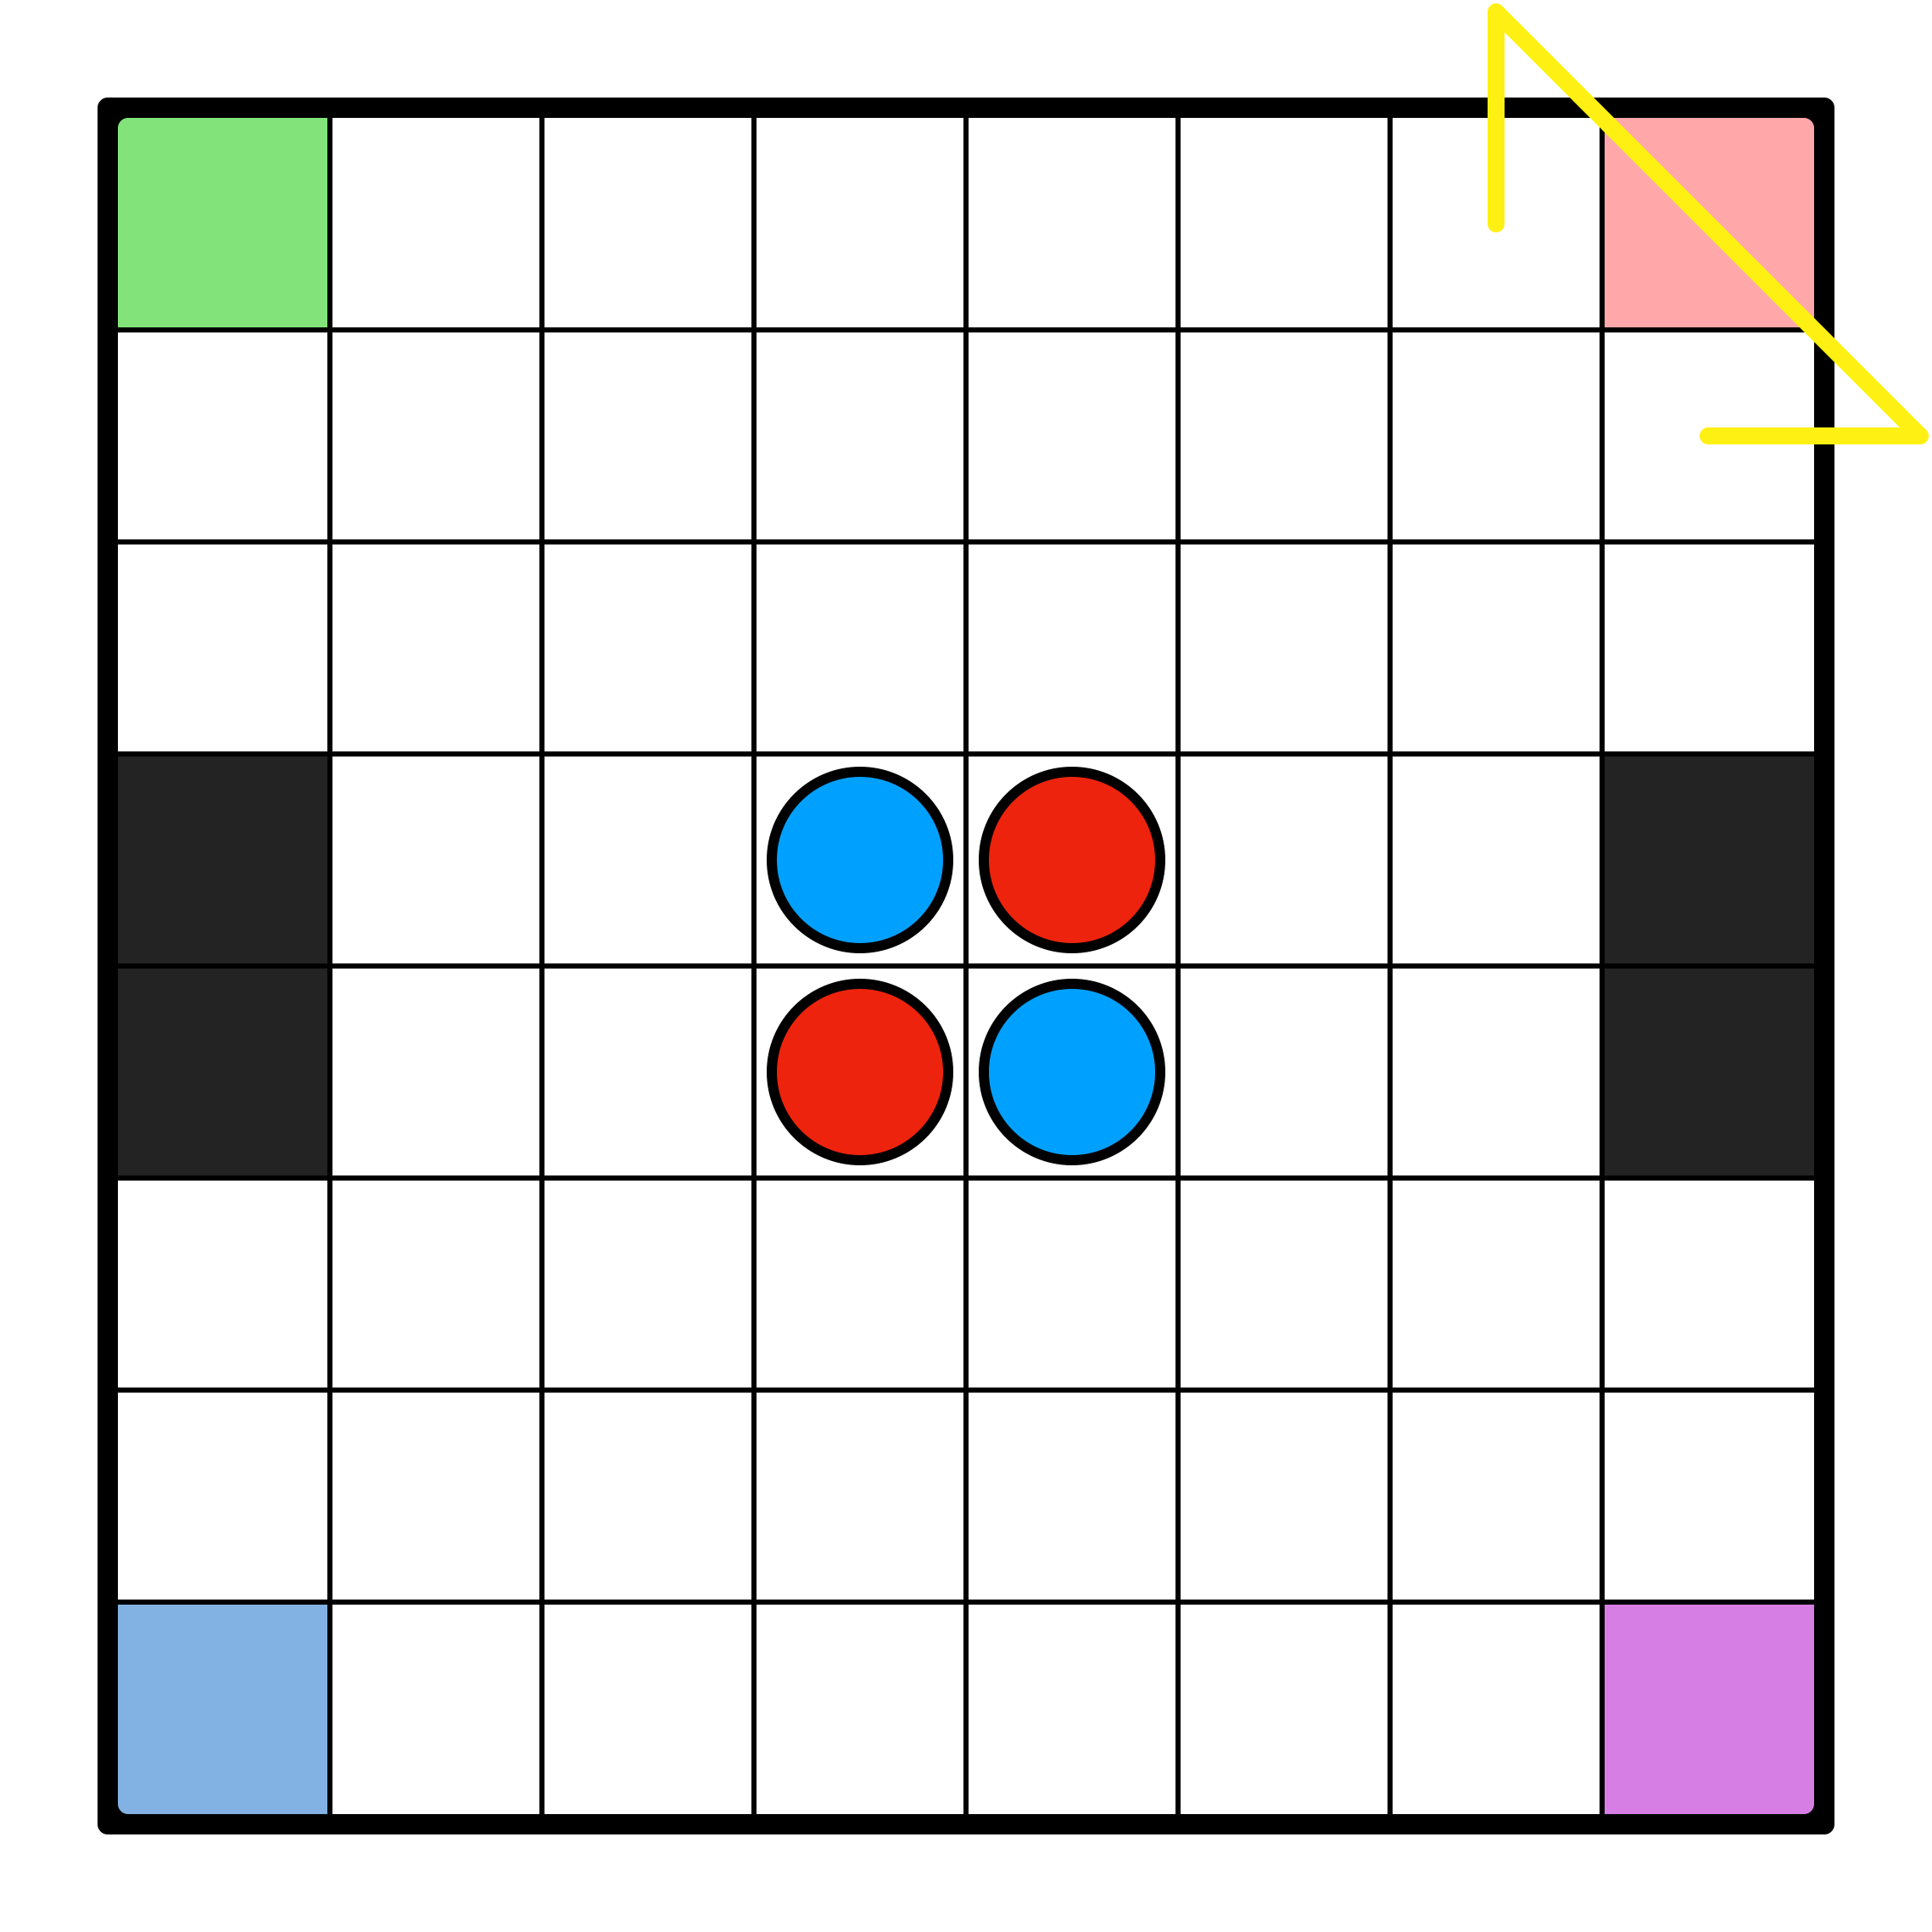
\includegraphics[width=0.5\linewidth]{pics/transition}
	\captionof{figure}[Transitionen]{ReversiXT Karte inkl. eingezeichneter Transition}
	\label{fig:reversixt-map}
\end{minipage}
\vspace{1em}

Eine weitere Besonderheit von ReversiXT sind \emph{Transitionen}.
Eine Transition kann an einem Feld liegen, an dem in einer gewissen Zugrichtung kein Weiteres mehr existiert.
Besitzt ein solches Feld nun eine Transition in einer Richtung, in die der Spieler durch einen Spielzug ziehen m\"ochte, kommt sein Stein an einer anderen festgelegten Stelle des Spielfeldes heraus.
Befindet sich nun ein Spieler auf dem siebten Feld in der ersten Reihe (siehe Abbildung~\ref{fig:reversixt-map}) und zieht nach oben, kommt er anschlie"send ganz rechts in der zweiten Reihe heraus.

Im Grundspiel Reversi gelten Ecken und die damit eingenommenen Kanten als sichere Felder, da es nicht mehr m\"oglich ist, diese durch einen g\"ultigen Zug umzuf\"arben.
Im Gegensatz dazu gibt es in ReversiXT aufgrund von \"Uberschreibsteinen keine sicheren Felder, da diese einfach \"uberschrieben werden k\"onnen.
Zus\"atzlich gibt es extrem viele Besonderheiten und unvorhersehbare Abh\"angigkeiten aufgrund von Transitionen und den zuvor genannten Zusatzregeln.
ReversiXT Karten m\"ussen zudem auch nicht zweidimensional sein, sondern k\"onnen h\"oherdimensionale Formen annehmen.
Dadurch kann man sich eine solche Karte auch nicht mehr als Brettspiel vorstellen, was dazu f\"uhrt, dass es nur sehr schwer nachvollziehbar ist, an welcher Stelle ein gewisser Spielzug endet.
Aus diesen Gr\"unden ist es f\"ur einen Menschen sehr schwer bis unm\"oglich ReversiXT erfolgreich gegen einen K.I.\ Client zu spielen.

\subsection{Vorstellung des Wahlpflichtfaches}\label{subsec:vorstellung-des-wahlpflichtfaches}
Die Aufgabe in diesem Modul besteht darin, einen Client mit einer k\"unstlichen Intelligenz zur bestm\"oglichen Spielzugwahl zu entwickeln, da es Computern m\"oglich ist, alle interessanten Spielz\"uge zu ber\"ucksichtigen und diese miteinander zu vergleichen.
Wir erwarten uns von diesem Fach, dass es dem Team einen \"Uberblick in die Entwicklung von k\"unstlicher Intelligenz gibt.
Zus\"atzlich ist es das erste Projekt im Studium, bei dem in einem Team an einem gemeinsamen Projekt gearbeitet wird.
Wir erhoffen uns damit wichtige Erfahrungen bez\"uglich Softwareplanung, Teamkoordination und Arbeitsverteilung zu sammeln, die f\"ur den sp\"ateren Berufseinstieg von gro"sem Nutzen sind.
Aktuell ist zudem das Thema maschinelles Lernen in aller Munde, wobei es nicht f\"ur jedes Projekt von Vorteil ist.
Bei maschinellem Lernen werden Programme mithilfe von Daten trainiert, um dann daraus gewisse Muster und Zusammenh\"ange selbst\"andig zu verstehen.
Damit nun z.B.\ eine Suchmaschine Katzenbilder von Hundebildern unterscheiden kann, muss sie vorab mit einer rie"sigen Menge solcher Bildern angelernt werden.
In Bereichen, in denen es kaum Daten f\"ur ein zu l\"osendes Problem gibt, oder bei dem die Daten zu sehr voneinander abweichen kann maschinelles Lernen nicht eingesetzt werden.
Betrachtet man nun ein Spiel wie ReversiXT und m\"ochte hier nun maschinelles Lernen einsetzen entsteht kein Problem aufgrund fehlender Daten, sondern es ergibt sich ein ganz anderes Problem.
Damit ein Computer selbstst\"andig lernt, wie man ReversiXT spielt, muss dieser alle M\"oglichkeiten von Spielz\"ugen durchgehen, um dann daraus R\"uckschl\"usse \"uber Z\"uge zu erhalten, die zu einem Sieg f\"uhren.
Nun gibt es aber so viele m\"ogliche Z\"uge, dass die Zeit nicht ausreicht um ein Spiel komplett durchsimulieren zu k\"onnen und vorallem hat man dann auch nur ein einziges Spiel simuliert, was selbstverst\"andlich alles andere als repr\"asentativ ist.
Mit der Entwicklung einer k\"unstlichen Intelligenz und einer Einf\"uhrung \"uber das maschinelle Lernen wollen wir die Vor- und Nachteile beider Innovationen erkennen und hautnah die Unterschiede verstehen lernen.


\bigskip
\newpage